\section{Genetic algorithm (GA) \cite{ai/book/Artificial-Intelligence-A-Modern-Approach/Russell-Norvig}}
\label{AI: Algorithms/Genetic algorithm (GA)}


\begin{figure}[H]
    \centering
    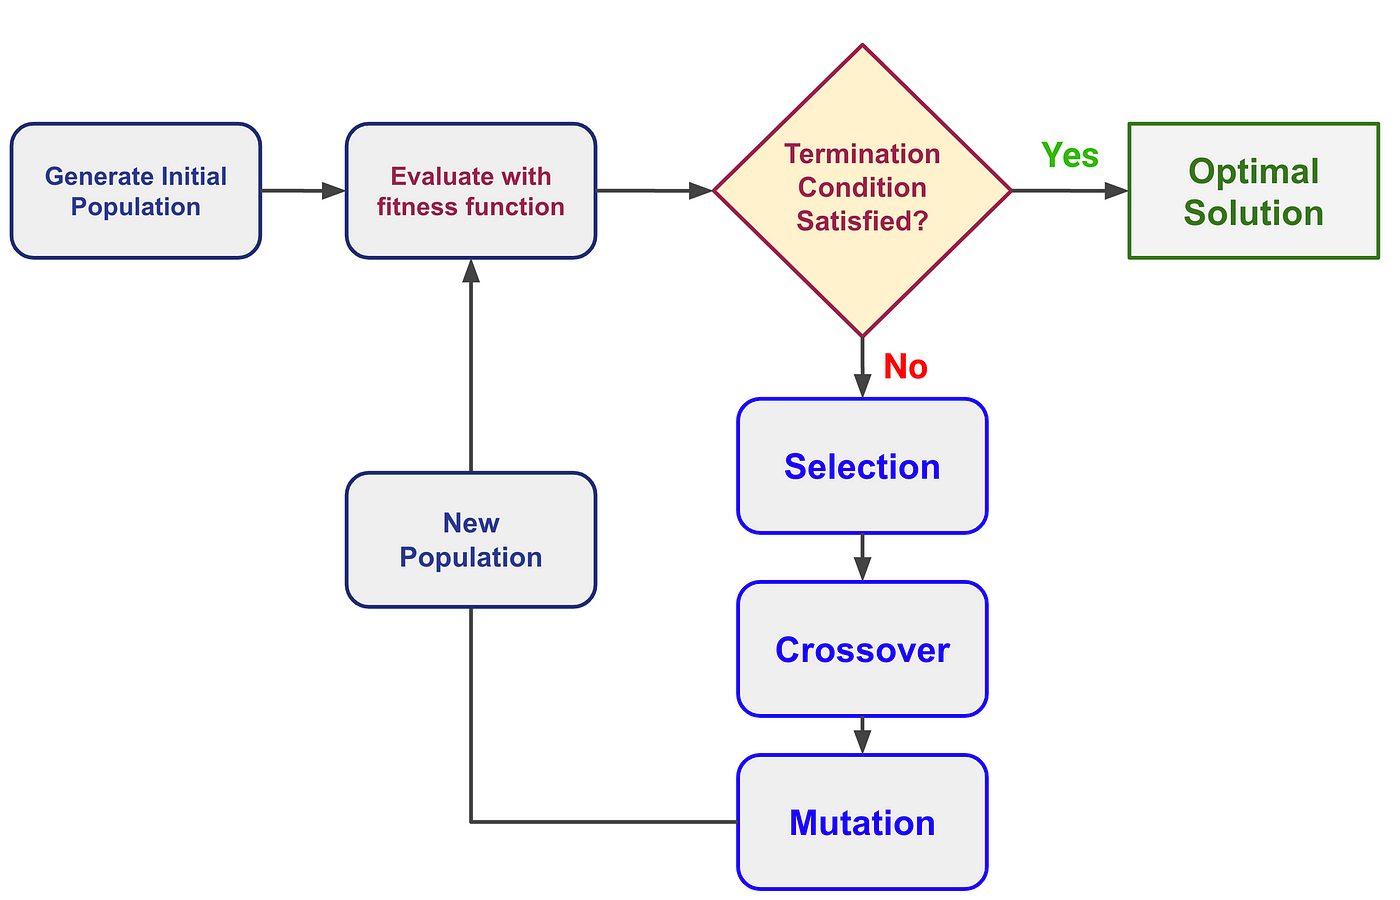
\includegraphics[
        width=\linewidth,
        height=6cm,
        keepaspectratio,
    ]{images/artificial-intelligence/searching/genetic-algorithm-flowchart.png}
    \caption{Genetic Algorithm - flowchart}
\end{figure}


\begin{enumerate}
    \item A genetic algorithm (GA) is a variant of stochastic beam search in which successor states are generated by combining \textit{two} parent states rather than by modifying a single state.
    \hfill \cite{ai/book/Artificial-Intelligence-A-Modern-Approach/Russell-Norvig}

    \item Like beam searches, GAs begin with a set of k randomly generated states, called the \textbf{population}.
    Each state, or \textbf{individual}, is represented as a string over a finite alphabet—most commonly, a string of $0$s and $1$s.
    \hfill \cite{ai/book/Artificial-Intelligence-A-Modern-Approach/Russell-Norvig}

    \item \textbf{culling}: all individuals below a given threshold are discarded, can be shown to converge faster than the random version
    \hfill \cite{ai/book/Artificial-Intelligence-A-Modern-Approach/Russell-Norvig}

    \item \textbf{steps}:
    \begin{enumerate}
        \item population states
        \hfill \cite{ai/book/Artificial-Intelligence-A-Modern-Approach/Russell-Norvig}

        \item each state is rated by the objective function, or (in GA terminology) the \textbf{fitness function}.
        A fitness function should return higher values for better states
        \hfill \cite{ai/book/Artificial-Intelligence-A-Modern-Approach/Russell-Norvig}

        \item two pairs are selected at \textbf{random} for \textbf{reproduction}, in accordance with the probabilities in (b).
        For each pair to be mated, a \textbf{crossover point} is chosen randomly from the positions in the string.
        \hfill \cite{ai/book/Artificial-Intelligence-A-Modern-Approach/Russell-Norvig}

        \item the offspring themselves are created by crossing over the parent strings at the crossover point.
        When two parent states are quite different, the crossover operation can produce a state that is a long way from either parent state.
        It is often the case that the population is quite diverse early on in the process, so crossover (like simulated annealing) frequently takes large steps in the state space early in the search process and smaller steps later on when most individuals are quite similar
        \hfill \cite{ai/book/Artificial-Intelligence-A-Modern-Approach/Russell-Norvig}

        \item each location (gene) is subject to random \textbf{mutation} with a small independent probability.
        \hfill \cite{ai/book/Artificial-Intelligence-A-Modern-Approach/Russell-Norvig}
    \end{enumerate}

    \item Like stochastic beam search, genetic algorithms combine an uphill tendency with random exploration and exchange of information among parallel search threads.
    \hfill \cite{ai/book/Artificial-Intelligence-A-Modern-Approach/Russell-Norvig}

    \item The primary advantage, if any, of genetic algorithms comes from the crossover operation.
    Yet it can be shown mathematically that, if the positions of the genetic code are permuted initially in a random order, crossover conveys no advantage.
    \hfill \cite{ai/book/Artificial-Intelligence-A-Modern-Approach/Russell-Norvig}

    \item \textbf{Schema}: Schema is a pattern or template where some positions are fixed (specified) and others are left open (unspecified).
    It's like a rule that only certain spots matter, and the rest can be anything.
    For example, in the pattern "246****", the first three positions (2, 4, 6) are fixed, and the last four can be any number or value.
    Genetic algorithms work best when schemata correspond to meaningful components of a solution.
    \hfill \cite{ai/book/Artificial-Intelligence-A-Modern-Approach/Russell-Norvig, common/online/chatgpt}

    \item \textbf{Instance}: An instance is a specific example that fits the schema.
    It follows the pattern by having the fixed parts the same as the schema but fills in the unspecified parts with actual values.
    For example, "24613578" is an instance of the schema "246****" because it has 2, 4, and 6 in the first three positions, and the rest are any values.
    \hfill \cite{ai/book/Artificial-Intelligence-A-Modern-Approach/Russell-Norvig, common/online/chatgpt}

    \item If the average fitness of the instances of a schema is above the mean, then the number of instances of the schema within the population will grow over time.
    This effect is unlikely to be significant if adjacent bits are totally unrelated to each other, because then there will be few contiguous blocks that provide a consistent benefit.
    \hfill \cite{ai/book/Artificial-Intelligence-A-Modern-Approach/Russell-Norvig}
\end{enumerate}




\begin{algorithm}[H]
    \caption{
        A genetic algorithm.
        In this more popular version, each mating of two parents produces only one offspring, not two.
        \cite{ai/book/Artificial-Intelligence-A-Modern-Approach/Russell-Norvig}
    }

    \SetKwFunction{FUNCTION}{\textsc{Reproduce}}
    \SetKwProg{Fn}{function}{ returns \normalfont{an individual}}{end}
    \Fn{\FUNCTION{$x, y$}}{
        \KwIn{$x, y$: parent individuals}

        $n \gets$ \textsc{Length}(x) \\
        $c \gets$ random number from $1$ to $n$ \\
        \Return \textsc{Append}( \\
            \hspace{0.5cm} \textsc{Substring}($x, 1, c$), \\
            \hspace{0.5cm} \textsc{Substring}($y, c+1, n$) \\
        )
    }


    \SetKwFunction{FUNCTION}{\textsc{Genetic-Algorithm}}
    \SetKwProg{Fn}{function}{ returns \normalfont{an individual}}{end}
    \Fn{\FUNCTION{$population$, \textsc{Fitness-Fn}}}{
        \KwIn{
            $population$: a set of individuals, \\
            \hspace{1cm}\textsc{Fitness-Fn}: a function that measures the fitness of an individual
        }
        \Repeat{some individual is fit enough, or enough time has elapsed}{
            $new\_population \gets \emptyset$\\
            \For{$i \gets 1$ \KwTo \textsc{Size}$(population)$}{
                $x \gets\text{ \textsc{Random-Selection}}(population, \text{\textsc{Fitness-Fn}})$\\
                $y \gets\text{ \textsc{Random-Selection}}(population, \text{\textsc{Fitness-Fn}})$\\
                $child \gets Reproduce(x, y)$\\
                \If{(small random probability)}{
                    $child \gets \text{\textsc{Mutate}}(child)$\\
                }
                add $child$ to $new\_population$\\
            }
            $population \gets new\_population$\\
        }
        \Return{the best individual in $population$, according to \textsc{Fitness-Fn}}
    }
\end{algorithm}













